\subsubsection{Secure Element} \label{subsection:counter-replace-encryption-key-local}
\subsubsection{Secure Element} \label{subsection:counter-replace-encryption-key-online}
\begin{figure}[h]
    \centering
    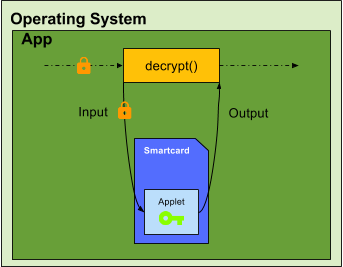
\includegraphics[width=0.8\textwidth]{data/encryptionKeySmart.png}
    \caption{Decryption by using a smartcard}
    \label{fig:encryptionKeySmart}
\end{figure}

%START TEXT INPUT
This is my real text! Rest might be copied or not be checked!
%START TEXT INPUT

can either be mounted in the sdcard slot or using an adapter for the usb interface
accessed over reads and writes to the filesystem
since it has to be small as a sd card and powered by the host system its hardware capabilities are restrained as well \cite{stSe} with power as low as 25MHz complexe calculations would take too much time

simple tasks (beschreiben)

unbestechlich, jedoch boolean abfrage immer crackbar, deswegen andere sachen machen zB verschlüsseln

encrypted strings from the application can be decrypted by the secure element
store property settings on it

encryption key can be stored on

no complexe tasks since low power


encryption inside app
x = encrypt("Hello")
function(x)

function(input):
y = decrypt(input) <- auf handy
case y == "Hello"

=> wenn falscher text dann random aktion/


am besten wäre die smartcard wenn kommunication über aussen geht, weil man da nichts faken kann bzw die app dann nicht funktionieren könnte, similar mit registriert auf dem server

\url{https://www.youtube.com/watch?v=rSH6dnUTDZo}
